\section{Date: 2026-09-08}
\noindent \textbf{Series ID: EMISSCO2TOTVTTCOUSA} 

\noindent This series is titled Total Carbon Dioxide Emissions From All Sectors, Coal for United States and has a frequency of Annual. The units are Million Metric Tons CO2 and the seasonal adjustment is Not Seasonally Adjusted.The observation start date is 1970-01-01 and the observation end date is 2021-01-01.The popularity of this series is 5. \\ 

\noindent \textbf{Series ID: COGANOPIMEPS} 

\noindent This series is titled Medical Services Expenditures by Disease: Other: Congenital Anomalies Price Index, MEPS Account Basis and has a frequency of Annual. The units are Index 2009=100 and the seasonal adjustment is Not Seasonally Adjusted.The observation start date is 2000-01-01 and the observation end date is 2020-01-01.The popularity of this series is 1. \\ 

\subsection{Raw Regression}
\noindent Regresses the two series against each other directly. A significant result here can come just as easily from both series sharing a long-run trend as from any real relationship.

\begin{center}
\begin{tabular}{lclc}
\toprule
\textbf{Dep. Variable:}                   & value\_fred\_COGANOPIMEPS & \textbf{  R-squared:         } &     0.606   \\
\textbf{Model:}                           &            OLS            & \textbf{  Adj. R-squared:    } &     0.585   \\
\textbf{Method:}                          &       Least Squares       & \textbf{  F-statistic:       } &     29.22   \\
\textbf{Date:}                            &      Tue, 08 Sep 2026     & \textbf{  Prob (F-statistic):} &  3.24e-05   \\
\textbf{Time:}                            &          15:27:44         & \textbf{  Log-Likelihood:    } &   -111.42   \\
\textbf{No. Observations:}                &               21          & \textbf{  AIC:               } &     226.8   \\
\textbf{Df Residuals:}                    &               19          & \textbf{  BIC:               } &     228.9   \\
\textbf{Df Model:}                        &                1          & \textbf{                     } &             \\
\textbf{Covariance Type:}                 &         nonrobust         & \textbf{                     } &             \\
\bottomrule
\end{tabular}
\begin{tabular}{lcccccc}
                                          & \textbf{coef} & \textbf{std err} & \textbf{t} & \textbf{P$> |$t$|$} & \textbf{[0.025} & \textbf{0.975]}  \\
\midrule
\textbf{const}                            &    -146.4574  &       51.777     &    -2.829  &         0.011        &     -254.827    &      -38.088     \\
\textbf{value\_fred\_EMISSCO2TOTVTTCOUSA} &       0.1533  &        0.028     &     5.406  &         0.000        &        0.094    &        0.213     \\
\bottomrule
\end{tabular}
\begin{tabular}{lclc}
\textbf{Omnibus:}       &  3.022 & \textbf{  Durbin-Watson:     } &    1.167  \\
\textbf{Prob(Omnibus):} &  0.221 & \textbf{  Jarque-Bera (JB):  } &    1.530  \\
\textbf{Skew:}          &  0.625 & \textbf{  Prob(JB):          } &    0.465  \\
\textbf{Kurtosis:}      &  3.429 & \textbf{  Cond. No.          } & 8.45e+03  \\
\bottomrule
\end{tabular}
%\caption{OLS Regression Results}
\end{center}

Notes: \newline
 [1] Standard Errors assume that the covariance matrix of the errors is correctly specified. \newline
 [2] The condition number is large, 8.45e+03. This might indicate that there are \newline
 strong multicollinearity or other numerical problems.

\begin{figure}
\centering
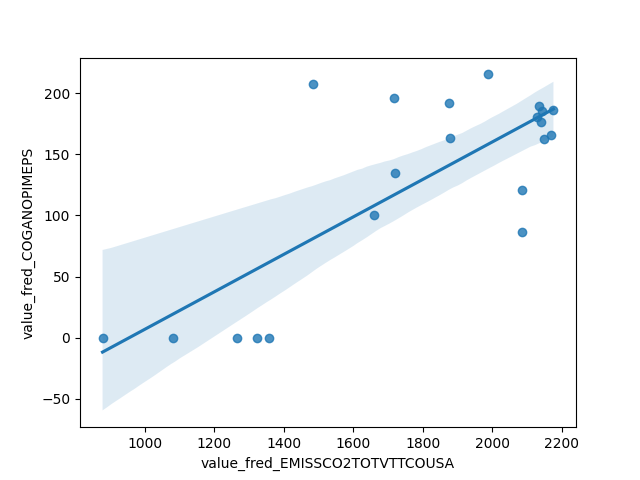
\includegraphics[scale = 0.9]{plots/plot_2026-09-08.png}
\caption{Raw Regression Plot for 2026-09-08}
\end{figure}
\newpage
\subsection{Detrended Regression}
\noindent Regresses the residuals of each series after removing its own linear time trend, so a shared trend can no longer drive the result on its own. A relationship that stays significant here is better evidence of a genuine link between the two series.

\begin{center}
\begin{tabular}{lclc}
\toprule
\textbf{Dep. Variable:}                              & value\_fred\_COGANOPIMEPS\_detrended & \textbf{  R-squared:         } &     0.559   \\
\textbf{Model:}                                      &                 OLS                  & \textbf{  Adj. R-squared:    } &     0.536   \\
\textbf{Method:}                                     &            Least Squares             & \textbf{  F-statistic:       } &     24.09   \\
\textbf{Date:}                                       &           Tue, 08 Sep 2026           & \textbf{  Prob (F-statistic):} &  9.76e-05   \\
\textbf{Time:}                                       &               15:27:44               & \textbf{  Log-Likelihood:    } &   -108.14   \\
\textbf{No. Observations:}                           &                    21                & \textbf{  AIC:               } &     220.3   \\
\textbf{Df Residuals:}                               &                    19                & \textbf{  BIC:               } &     222.4   \\
\textbf{Df Model:}                                   &                     1                & \textbf{                     } &             \\
\textbf{Covariance Type:}                            &              nonrobust               & \textbf{                     } &             \\
\bottomrule
\end{tabular}
\begin{tabular}{lcccccc}
                                                     & \textbf{coef} & \textbf{std err} & \textbf{t} & \textbf{P$> |$t$|$} & \textbf{[0.025} & \textbf{0.975]}  \\
\midrule
\textbf{const}                                       &   -6.734e-12  &        9.567     & -7.04e-13  &         1.000        &      -20.023    &       20.023     \\
\textbf{value\_fred\_EMISSCO2TOTVTTCOUSA\_detrended} &       0.3032  &        0.062     &     4.908  &         0.000        &        0.174    &        0.432     \\
\bottomrule
\end{tabular}
\begin{tabular}{lclc}
\textbf{Omnibus:}       &  4.692 & \textbf{  Durbin-Watson:     } &    1.541  \\
\textbf{Prob(Omnibus):} &  0.096 & \textbf{  Jarque-Bera (JB):  } &    2.578  \\
\textbf{Skew:}          &  0.726 & \textbf{  Prob(JB):          } &    0.276  \\
\textbf{Kurtosis:}      &  3.915 & \textbf{  Cond. No.          } &     155.  \\
\bottomrule
\end{tabular}
%\caption{OLS Regression Results}
\end{center}

Notes: \newline
 [1] Standard Errors assume that the covariance matrix of the errors is correctly specified.

\begin{figure}
\centering
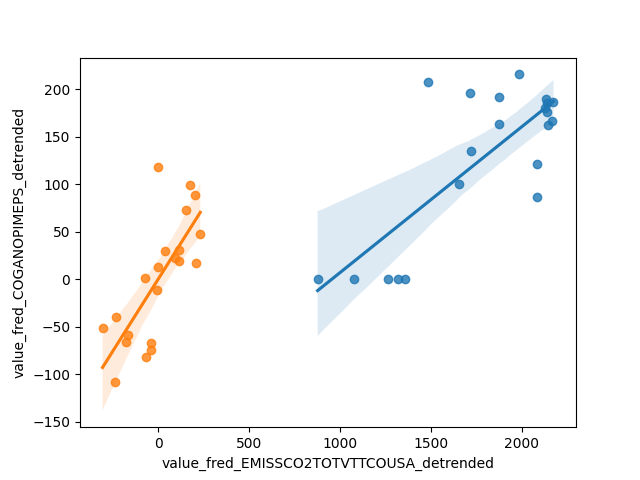
\includegraphics[scale = 0.9]{plots/plot_2026-09-08_detrended.png}
\caption{Detrended Regression Plot for 2026-09-08}
\end{figure}
\newpage
